\documentclass[11pt]{amsart}

%you can add extra packages if you need them
\usepackage{amsfonts,amssymb,amscd,amsmath,enumerate,verbatim,calc,thumbpdf,mathrsfs, graphicx, multicol, multirow}

\setlength{\oddsidemargin}{0.25in}  %please do not change
\setlength{\evensidemargin}{0.25in} %please do not change
\setlength{\marginparwidth}{0in} %please do not change
\setlength{\marginparsep}{0in} %please do not change
\setlength{\marginparpush}{0in} %please do not change
\setlength{\topmargin}{0in} %please do not change

\setlength{\footskip}{.3in} %please do not change
\setlength{\textheight}{8.75in} %please do not change
\setlength{\textwidth}{6in} %please do not change
\setlength{\parskip}{4pt} %please do not change

\theoremstyle{plain}%default
\newtheorem{thm}{Theorem}[section]
\newtheorem{lem}[thm]{Lemma}
\newtheorem{cor}[thm]{Corollary} 
\newtheorem{prop}[thm]{Proposition}
\newtheorem{remark}[thm]{Remark}
\newtheorem{mythm}[thm]{My Great Result}

\theoremstyle{definition}
\newtheorem{defin}[thm]{{Definition}}
\newtheorem{ex}[thm]{Example}

\theoremstyle{remark}
\newtheorem{rem}[thm]{Remark}

\numberwithin{equation}{thm}

\begin{document}

\title[RNA Secondary Structures]{Counting RNA Secondary Structures Using Analytic Combinatorics}
\thanks{Adviser: Dr. Torin Greenwood}
\author[Burnham]{Kaleb Burnham}

\address{Department of Mathematics 2750\\ North Dakota State University\\PO BOX 6050\\ Fargo, ND 58108-6050\\ USA}

\email{kaleb.burnham@ndsu.edu}

\begin{abstract}
Ribonucleic acids (RNA) are critical molecules for the coding, decoding, regulation, and the expression of genes. Due to their necessity for all forms of life, the ways that each molecule folds unto itself is of great research interest. A challenge in this field is predicting which structures a given RNA molecule will fold into. This paper will compute by construction the number of possible secondary structures of a sequence of arbitrary length, then utilize grammars and generating functions to compute the asymptotic growth of the space as the length increases.
\end{abstract}

\maketitle
%\setcounter{page}{***} Please do not change this line

\section{Introduction}
Given any RNA strand, it is of great interest to predict its possible secondary structures. In molecular biology, the structure of a given molecule encodes information about its function. Conversely, a molecule with a specific function (and hence, a specific structure) may be desired, as in gene therapy. Researchers then would look for an RNA sequence that folds into the desired structure. Significant progress has been made in these fronts in recent decades. In many cases, researchers are able to closely predict structures. However, these predictions are made on a case-by-case basis
and it remains difficult to predict structures for some classes of RNA. Nevertheless, it can be useful to look for patterns between different strands to design useful models.

To help describe RNA folding, researchers consider three structures of a molecule. A molecule's primary structure is the one dimensional string describing its nucleotide makeup. Since the most common nucleotides are adenine, guanine, cytosine, and uracil, this is simply a string from the alphabet {A, G, C, U}. Its secondary structure is the hypothetical two-dimensional structure as the string bends and folds in on itself as determined by the pairing of its constituent nucleotides. Watson-Crick base pair rules specify that A binds with U and G binds with C. However, these are not strict rules. It has been observed that a pairing between any of these nucleotides may occur, as well as pairing with another nucleotide, hypoxanthine. Due to these complexities, we will ignore the constituent nucleotides in each pairing for our enumeration technique. The third structure is the final, three-dimensional structure that encodes the functional information about the molecule. In reality, the transitions between stages are not well-defined and happen simultaneously. By breaking the problem down to secondary structures, it is possible to search for basic patterns between differing RNA molecules in an attempt to create models to describe their final tertiary structure. A natural first question in this search is with regards to the search space: How many possible secondary structures exist for a given RNA strand?

\section{Preliminaries}
\begin{defin}
    Let $A$ be the alphabet $\{A, C, G, U\}$. Let $a_1a_2a_3...a_n$ be a string of nucleotides where each $a_i \in A$. We say that a \textit{secondary structure} is a collection of pairings between nucleotides such that a pairing between any two nucleotides $a_j, a_k, j < k$ is valid if for any other pairing $a_l, a_m, l < m$, it is the case that $j < l < m < k$ or $j < k < l < m$ or $l < m < j < k$. Additionally, we restrict each nucleotide to be paired to at most one other nucleotide.
\end{defin}

\begin{figure}[htp]
    \centering
    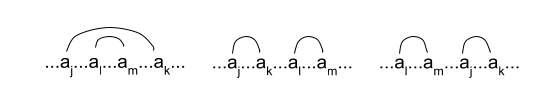
\includegraphics[width=11cm]{PairingDef.png}
    \caption{The three possibilities for any two pairings. Notice that none of the pairing lines cross others.}
    \label{fig:definition}
\end{figure}

Since we are only counting the number of possible secondary structures, it does not matter for our purposes what the specific nucleotides are at each point - we are only concerned if they are paired with another nucleotide. This allows us to simplify our model further by designating a period for an unpaired nucleotide, a left parenthesis for a new bond, and a right parenthesis to close a bond. Figure \ref{fig:dotbracketnotation} provides an example of this.

\begin{figure}[htp]
    \centering
    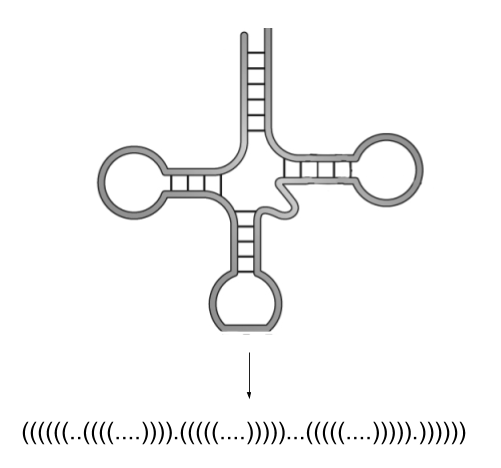
\includegraphics[width=10cm]{2Dto1D.png}
    \caption{Dot-Bracket Notation}
    \label{fig:dotbracketnotation}
\end{figure}

This notation introduces a new yet similar question: given a string of length $n$, how many ways can we place $k$ pairs of parentheses such that every left parenthesis is matched with a right, and, counting from left to right, the number of right parentheses never exceeds the number of left parentheses? Without considering specific nucleotides, this will give us the number of possible secondary structures of any arbitrary length string.

\section{Dyck and Motzkin Languages}

First, consider the string of only parentheses which follows the rules from the previous paragraph. From now on, these will be referred to as \textit{Dyck words}.

\begin{defin}
    A \textit{Dyck word} is a balanced string of parentheses such that, when reading left to right, there are never more right parentheses than left parentheses at any position.
\end{defin}

\begin{thm}
    \label{DyckWords}
    The number $C_k$ of Dyck words of length $2k$ is $\binom{2k}{k}\cdot\frac{1}{k+1}$.
\end{thm}

\begin{proof}
    Define $S$ to be the set of strings of length $2k$ with $k$ lefts and $k$ rights with the condition that the number of lefts exceeds the number of rights at some point. So, $S$ is the set of balanced strings that are not Dyck words.
    Define $T$ to be the set of strings of length $2k$ with $k-1$ lefts and $k+1$ rights. Choosing $k-1$ lefts and letting the rest be rights means that $|T| = \binom{2k}{k-1}$. A bijection will be shown between $S$ and $T$.

    Let $\tau$ be defined on all strings of parentheses. Its operation is defined such: $\tau(s)$ means to traverse the string left to right. At the first symbol $p_0$ where the number of rights exceeds the number of lefts, flip all the remaining parentheses, not including $p_0$.

    For any $s \in S$, $\tau(s)$ produces a string with $k-1$ lefts and $k+1$ closes. Thus, $\tau(s) \in t$ and $\tau: S \rightarrow T$ is injective. Similarly, for any $t \in T$, $\tau(t) \in S$. So, $\tau: T \rightarrow S$ is injective. Since $\tau$ is injective both ways, there exists a bijection between $S$ and $T$. Therefore, $|S| = |T| = \binom{2k}{2k-1}$. Hence, the number of Dyck words of length $2k$ is $\binom{2k}{k} - \binom{2k}{k-1}.$

    \begin{align*}
        \binom{2k}{k} - \binom{2k}{k-1} &= \frac{(2k)!}{k!k!} - \frac{(2k)!}{(k-1)!(k+1)!}\\
        &= (2k)!\cdot\left(\frac{1}{k!k!} - \frac{1}{(k-1)!(k+1)!}\right)\\
        &= (2k)!\cdot\left(\frac{k+1}{k!(k+1)!} - \frac{k}{k!(k+1)!}\right)\\
        &= (2k)!\cdot\left(\frac{1}{k!(k+1)!}\right)\\
        &= \frac{(2k)!}{k!k!}\cdot\frac{1}{k+1}\\
        &= \binom{2k}{k}\cdot\frac{1}{k+1}
    \end{align*}
\end{proof}

Conveniently, the sequence ${C_i}, i \geq 0$ corresponds exactly with the Catalan numbers! From here, we need to mix in dots with the parentheses and observe how that changes the sequence. Strings of dots and parentheses will now be called \textit{Motzkin words}.

\begin{defin}
A \textit{Motzkin word} is a string of dots and parentheses such that the parentheses form a Dyck word.
\end{defin}

\begin{thm}
    The number $M(n)$ of Motzkin words of length $n$ is 
    $$\sum_{k=0}^{\lfloor \frac{n}{2}\rfloor} \binom{n}{2k} \cdot C_k.$$
\end{thm}

\begin{proof}
    This will be proven by construction of all Motzkin words. Consider $n$ positions. Each position must be either a dot or parenthesis. Clearly, the number of parentheses must be even and less than or equal to $n$. The positions that do not contain a parenthesis will contain a dot. So, the number of ways to select the positions with parentheses is
    
    $$\binom{n}{0} + \binom{n}{2} + \binom{n}{4} + ... + \binom{n}{2\cdot\lfloor\frac{n}{2}\rfloor}= \sum_{k=0}^{\lfloor \frac{n}{2}\rfloor} \binom{n}{2k}.$$
    
    Now, each parenthesis must still chosen such that the string of parentheses forms a Dyck word. Theorem \ref{DyckWords} gives us the number of ways to do this. So, the total number of Motzkin words of length $n$ is
    
    $$\binom{n}{0}C_0 + \binom{n}{2}C_1 + \binom{n}{4}C_2 + ... + \binom{n}{2\cdot\lfloor\frac{n}{2}\rfloor}C_{\lfloor\frac{n}{2}\rfloor} = \sum_{k=0}^{\lfloor \frac{n}{2}\rfloor} \binom{n}{2k}C_k.$$
\end{proof}

So, we have found the number of Motzkin words of length $n$, and hence the number of secondary structures of an RNA molecule with $n$ nucleotides. This function $M(n)$ coincides with the $n^{th}$ Motzkin number, and the first 15 numbers are: 1, 1, 2, 4, 9, 21, 51, 127, 323, 835, 2188, 5798, 15511, 41835, 113634. They appear to grow extremely rapidly, but their growth rate is not obvious. So, it could be of use to analyze their asymptotic growth. To do this, we will need more complex machinery: context-free grammars and generating functions.

\section{Context-Free Grammars}
A context-free grammar is a formal grammar with a set of rules that can describe any string in a language. A formal definition is provided.

\begin{defin}[\cite{Sipser}]
A context-free grammar is a 4-tuple $(V, \sum, R, S)$, where
    \begin{enumerate}
        \item$V$ is a finite set called the variables,
        \item$\sum$ is a finite set, disjoint from $V$, called the terminals,
        \item$R$ is a finite set of rules, with each rule being a variable and a string of variables and terminals, and
        \item$S \in V$ is the start variable.
    \end{enumerate}
\end{defin}

A grammar $G$ that describes Dyck words is simple and has only one production rule: 

$$S\rightarrow (S)S\ |\ \emptyset.$$

Using this grammar allows us to create a parse tree for any Dyck word. Consider the string $(()())()$; Figure \ref{fig:parsetree} shows its corresponding parse tree.

\begin{figure}[htp]
    \centering
    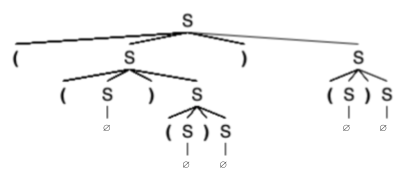
\includegraphics[width=10cm]{ParseTree.png}
    \caption{A parse tree for the string $(()())()$.}
    \label{fig:parsetree}
\end{figure}

To read the output of the parse tree, traverse the leaves left to right, skipping over the empty string $\phi$. If each word has only one possible parse tree and we can find a way to count the number of parse trees generated by a grammar, we can count the total number of words of any length in our desired format. To verify there is only one parse tree per word, we need to check this grammar is not \textit{ambiguous}.

\begin{defin}[\cite{Sipser}]
If a grammar generates the same word with different parse trees, we say that the word is derived \textit{ambiguously} in the grammar. If a grammar generates some word ambiguously, we say that the grammar is \textit{ambiguous}.
\end{defin}

Showing the grammar is unambiguous is equivalent to showing that every word has a unique decomposition

\begin{thm}
\label{GUnambiguous}
The output of $G: S \rightarrow (S)S\ |\ \emptyset$ is the set of all Dyck words, and every Dyck word can be produced in exactly one way.
\end{thm}

\begin{proof}
Define a primitive string as one where the number of lefts equals the number of rights only at the end of the string. Take any Dyck word $s$. Inductively, assume that any Dyck word shorter than $s$ has a single parse tree (the empty string has a single parse tree, so the base case is unambiguous). If $s$ is a primitive string, then it has a unique decomposition to $(s')$, where $s'$ is not necessarily primitive. If $s$ is not primitive, we need to find an unambiguous way to decompose $s$ into $s_1$ and $s_2$ so that $s = (s_1)s_2$. Any position where $s$ is split must also have an equal number of rights and lefts. Suppose $s$ is decomposed at the first position where rights equal lefts, making $s_1$ a primitive string. Then both $s_1$ and $s_2$ are shorter than $s$ and each have a single parse tree. Combining the parse trees of $s_1$ and $s_2$ gives one parse tree for $s$.

Now consider the other possibilities that would make $s_1$ a non-primitive string. Then $s_1$ has a notion of a last primitive string. But, the decomposition to $(s_1')$ implies the last primitive string would contain one extra left parenthesis making it unbalanced. Thus, $G$ has only a single possible parse tree for any Dyck word.

We have just shown that all Dyck words can be described using grammar $G$. Now, it must be shown that the grammar generates exactly Dyck words and nothing else. 

Since each use of the production rule $S$ introduces both a single left and right parenthesis, $G$ generates words with balanced parentheses. Additionally, for each subsequent use, the new pair of parentheses is either wholly contained within another pair, or is concatenated to the end. So, it cannot be the case that one parenthesis is contained within a pair, and the other is outside the same pair. Thus, any word produced by $G$ is a Dyck word.
\end{proof}

This result implies that if we count the total number of outputs of this grammar, that number is exactly the number of Dyck words. In the next section, we will find a generating function that can do this. But first, let us find a grammar for Dyck words with dots.

One way to do this is to create a new production rule $T$ and modify the original rule $S$. So, a new grammar might be

\begin{align*}
S &\rightarrow T(S)S\ |\ T\\
T &\rightarrow .T\ |\ \emptyset
\end{align*}

It can be observed that these rules still force balanced parentheses and allow for an arbitrary number of dots at the beginning, end, and between any pair. However, there is a simpler grammar that is equivalent. Call this grammar $H$.

\begin{align*}
S \rightarrow .S\ |\ (S)S\ |\ \emptyset
\end{align*}

It must be shown that $H$ is unambiguous and describes exactly all Motzkin words.

\begin{thm}
The output of $H: S \rightarrow .S\ |\ (S)S\ |\ \emptyset$ is the set of all Motzkin words, and every Motzkin word can be produced in exactly one way.
\end{thm}

\begin{proof}
Similar to Theorem \ref{GUnambiguous}, define a primitive word as one where the number of lefts equals the number of rights only at the end of the word. In this case, dots are allowed in the word. Take any Motzkin word $m$. There are two cases for $m$: either $m$ begins with a dot or $m$ begins with a left parenthesis. If $m$ begins with a dot, then the only way to decompose $m$ is into $.m'$, where $m'$ is $m$ without the first dot. If $m$ begins with a left parenthesis, then using the same argumentation as Theorem \ref{GUnambiguous}, $m$ can be uniquely decomposed to $(m_1)m_2$. Thus, $H$ produces a single possible parse tree for any Motzkin word.

We have placed no limitations on the placement of dots. When parentheses are introduced, they are introduced as a pair which is either wholly contained within another pair, or is concatenated to the end. Again, the same argumentation as Theorem \ref{GUnambiguous} shows the output of $H$ is exactly the set of Motzkin words.
\end{proof}

\section{Generating Functions}
To count the number of parse trees created by each grammar, we will utilize an object called a generating function.

\begin{defin}[\cite{Wilf}]
\label{genfundef}
A \textit{generating function} for the sequence $(a_n)$ is the power series $\sum_{n \geq 0} a_nx^n$. This means the numbers in $(a_n)$ correspond to the coefficients in the power series.
\end{defin}

Generating functions are useful because they allow us to study sequences in terms of polynomials and calculus. Often, they can find an exact formula for the numbers in a sequence, as we will see in a moment. Other areas they can help with include

\begin{itemize}
    \item Compute statistical properties of a sequence
    \item Finding asymptotic formulas
    \item Proving convexity
    \item Proving identities
\end{itemize}

\begin{ex}
Take the recurrence equation for Fibonacci sequence.

$$ F_{n+1} = F_n + F_{n-1}$$

The first few terms of this sequence are 1, 1, 2, 3, 5, 8, 13, 21, 34, 55, 89. This alone does not tell us much about the sequence. If we want to find an exact formula or attempt to statistically analyze this sequence, generating functions can help!

Using Definition \ref{genfundef}, the power series we would look for is $1 + x + 2x^2 + 3x^3 + 5x^4 + 8x^5 + 13x^6 + 21x^7 + ...$. Conveniently, this is the expansion of the function $F(x) = \frac{1}{1-x-x^2}$ about the origin! In this case, $F(x)$ is said to be the generating function for the Fibonacci numbers.

By performing a partial fraction decomposition and some algebra, an explicit formula for the coefficients can be found: $F_n = \frac{1}{\sqrt{5}}\left[\left(\frac{1+\sqrt{5}}{2}\right)^{n} -\left(\frac{1-\sqrt{5}}{2}\right)^{n}\right]$.

\end{ex}

We have already claimed that generating functions count objects. What happens if we want to count objects from differing sets?

\begin{ex}

How many ways are there to make a sum of 10, using one element from each of the following sets: {2, 3, 6, 7} and {3, 4, 5, 8}?

The first set is represented by the generating function $x^2 + x^3 + x^6 + x^7$, since there is one way to make a sum of 2 in the first set, one way to make a sum of 3, etc. The second set is represented by the generating function $x^3 + x^4 + x^5 + x^8$ using the same reasoning. Considering the sum of these functions, we have 

$$(x^2 + x^3 + x^6 + x^7)\cdot(x^3 + x^4 + x^5 + x^8)$$

$$= x^5 + 2x^6 + 2x^7 + x^8 + x^9 + 3x^{10} + 3x^{11} + x^{12} + x^{14} + x^{15}.$$

To find the answer we only need to look at the coefficient of the term with an exponent of 10, which is 3. Thus, there are three ways to make a sum of 10 using one element from each of the sets.
\end{ex}

In general, we have a set counted by the generating function $A(x)$ and a set counted by the generating function $B(x)$. The ways to pick one object from each set while tracking the total size is $A(x) \cdot B(x)$. We'll prove it.

\begin{prop}
\label{CauchyProduct}
Let $A(x) = \sum_{n>=0} a_ix^n$ and $B(x) = \sum_{n>=0} b_ix^n$ be two infinite power series. Then, $A(x) \cdot B(x) = \sum_{n\geq0}(\sum_{k=0}^{n}a_kb_{n-k})x^n$.
\end{prop}

\begin{proof}
    \begin{align*}
        A(x) \cdot B(x) &= \left(\sum_{n\geq0} a_nx^n\right)\left(\sum_{n\geq0} b_nx^n\right)\\
        &= (a_0 + a_1x + a_2x^2 + ...)(b_0 + b_1x + b_2x^2 + ...)\\
        &= a_0b_0 + (a_0b_1 + a_1b_0)x + (a_0b_2 + a_1b_1 + a_2b_0)x^2 + ...\\
        &= \sum_{n\geq0}\left(\sum_{k=0}^{n}a_kb_{n-k}\right)x^n
    \end{align*}
\end{proof}

The grammar $G$ essentially says that any non-empty Dyck word can be broken into two Dyck words of total length $n-2$ plus two parentheses. Since we are counting the number of Dyck words, Proposition \ref{CauchyProduct} hints that we should see an $S(x)^2$ term in the next proof.

\begin{thm}
    The generating function that counts the parse trees of the grammar $G: S \rightarrow (S)S\ |\ \emptyset$ 
    is $S(x) = \frac{1 - \sqrt{1-4x}}{2x}$.
\end{thm}

\begin{proof}
    Let $S(x) = \sum_{n \geq 0}{c_nx^n}$ be the generating function corresponding to the number of Dyck words with $n$ pairs. If $n = 0$, then $c_0 = 1$. Consider the case when $n > 1$. Since the grammar G defines the exact location for one pair, the coefficient $c_n$ corresponds to the number of combinations of valid parenthesizations of the first and second S. Thus, $c_n = \sum_{k=1}^{n}c_{k-1}c_{n-k}$. Plugging this value into the first equation gives 

    $$S(x) = \sum_{n \geq 0} \left( \sum_{k=1}^{n}c_{k-1}c_{n-k}\right) x^n.$$

    By moving an $x$ to the front of the sums and re-indexing, this can be re-written as

    \begin{align*}
        S(x) &= \sum_{n \geq 0} \left( \sum_{k=1}^{n}c_{k-1}c_{n-k}\right) x^n\\
        &= x\sum_{n \geq 0} \left( \sum_{k=1}^{n}c_{k-1}c_{n-k}\right) x^{n-1}\\
        &= x\sum_{n \geq 0} \left( \sum_{k=0}^{n-1}c_{k}c_{n-(k+1)}\right) x^{n-1}\\
        &= x\sum_{n \geq 0} \left( \sum_{k=0}^{n}c_{k}c_{n-k}\right) x^{n}\\
    \end{align*}

    Note that this double sum is equivalent to $S(x)^2$ as shown in Proposition \ref{CauchyProduct}. We still need to add one for when $n = 0$. So, we can write the full equation as $S(x) = xS(x)^2 + 1$. Solving for $S(x)$, we obtain $S(x) = \frac{1 \pm \sqrt{1 - 4x}}{2x}$.

    If we use the addition sign, we arrive at the undefined value $\frac{2}{0}$, meaning that as $x \to 0$, $S(x) \to \infty$. This is clearly incorrect. By convention, there is only $1$ string with length $0$. Using the minus sign gives $\frac{0}{0}$, an indeterminate form. Using L'Hospital's rule, we get

    \begin{align*}
        S(0) &= \lim_{x\to0}\frac{1 - \sqrt{1 - 4x}}{2x}\\
        &= \lim_{x\to0}\frac{\frac{d}{dx}(1-\sqrt{1-4x})}{\frac{d}{dx}(2x)}\\
        &= \lim_{x\to0}\frac{2}{2\sqrt{1-4x}}\\
        &= 1.
    \end{align*}

    \noindent which is exactly what was desired. Thus, we have our generating function: $S(x) = \frac{1 - \sqrt{1-4x}}{2x}$.
\end{proof}

Take a moment to compare the grammar $G: S \rightarrow (S)S\ |\ \emptyset$ to an equation arrived at in the previous proof: $S(x) = xS(x)^2 + 1$. It appears that for each pair of parentheses we add to the word, we place an $x$ and multiply it by $S(x)^2$ since we have two $S$ terms. Then, we add one since, by convention, there is exactly one empty word. In fact, this is exactly what is happening; it is a result of the Chomsky–Schützenberger enumeration theorem which transforms unambiguous context-free grammars to a system of equations. In our case, we only have one equation because the grammar has a single rule. A \textit{statistic} is the object that a generating function counts, and in the previous case we were counting pairs of parentheses.

\begin{thm}
    The generating function that counts the parse trees of the grammar $S \rightarrow .S\ |\ (S)S\ |\ \emptyset$ is $S \rightarrow (S)S\ |\ \emptyset$ is $S(x) = \frac{1-x - \sqrt{-3x^2 - 2x + 1}}{2x^2}$.
\end{thm}

\begin{proof}
    Using the Chomsky–Schützenberger enumeration theorem, we can quickly derive an equation for $S(x)$. In this case, our statistic will be a single character - either a dot, left, or right parenthesis. So for each term that adds characters, we multiply by $x$ for each character that is introduced - introducing a pair of parentheses now results in $x^2$. We can quickly arrive at the formulation $S(x) = xS(x) + x^2S(x)^2  + 1$. Solving for $S(x)$,


    $$x^2S(x)^2 + (x-1)S(x) + 1 = 0$$
    \begin{align*}
    \Rightarrow S(x) &= \frac{1-x \pm \sqrt{(x-1)^2 - 4x^2}}{2x^2}\\
    \Rightarrow S(x) &= \frac{1-x \pm \sqrt{-3x^2 - 2x + 1}}{2x^2}
    \end{align*}
    
    Again, a plus or minus operation must be chosen for the generating function. By picking the plus operation, we again see that $S(0)$ gives $\frac{2}{0}$, but the minus allows $S(0) = \frac{0}{0}$. Two doses of L'Hospital should give one.

    \begin{align*}
        S(0) &= \lim_{x\to0}\frac{1-x - \sqrt{-3x^2 - 2x + 1}}{2x^2}\\
        &= \lim_{x\to0}\frac{\frac{d^2}{dx^2} \left(1-x - (-3x^2 - 2x + 1)^{1/2}\right)}{\frac{d^2}{dx^2}2x^2}\\
        &= \lim_{x\to0}\frac{\frac{d}{dx}\left(-1-\frac{-6x-2}{2\sqrt{-3x^2-2x+1}}\right)}{\frac{d}{dx}4x}\\
        &= \lim_{x\to0}\frac{\frac{4}{(-3x^2-2x+1)^{3/2}}}{4}\\
        &= \lim_{x\to0}\frac{\frac{4}{1}}{4}\\
        &= 1.
    \end{align*}
    
    Indeed, it does. So, the generating function is $S(x) = \frac{1-x - \sqrt{-3x^2 - 2x + 1}}{2x^2}$
\end{proof}

\section{Asymptotic Analysis}

At this stage, we have the generating function $S(x)$. All that is left now is to extract the coefficients of the Taylor series expansion. To do this, we utilize the following theorem.

%\begin{prop}
%\label{Flajolet-Odlyzko Proposition}
%The binomial coefficients expressing $[x^n](1-x)^\alpha$ have an asymptotic expansion as $n \to \infty$,
%
%$$[x^n](1-x)^\alpha \sim \frac{n^{-\alpha-1}}{\Gamma(-a)}, \alpha \notin \{0, 1, 2, ...\}.$$
%\end{prop}

\begin{thm}[Flajolet-Odlyzko \cite{Flajolet}]
\label{F-O}
Assume that, with the sole exception of the singularity $z = 1$, $f(z)$ is analytic in the domain $\Delta = \Delta(\phi, \eta)$, where $\eta > 0$ and $0 < \phi < (\pi/2)$. Assume further that as $z$ tends to 1 in $\Delta$,

$$ f(z) \sim (1-z)^\alpha,$$

for some real number $\alpha$. Then the $n^{th}$ Taylor coefficient of $f(z)$ satisfies

$$ f_n = [z^n]f(z) \sim \frac{n^{-\alpha-1}}{\Gamma(-\alpha)}.$$

\begin{figure}[htp]
    \centering
    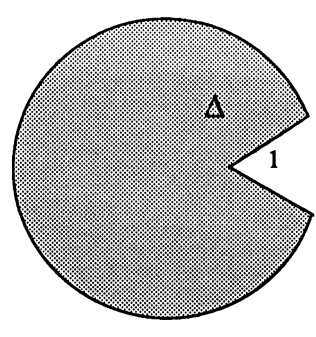
\includegraphics[width=4cm]{FlajoletDomain.png}
    \caption{The domain $\Delta(\phi, \eta)$. \cite{Flajolet}}
    \label{fig:flajoletdomain}
\end{figure}
\end{thm}

We have already shown that the generating function $S(x) = \frac{1-x - \sqrt{-3x^2 - 2x + 1}}{2x^2}$ is continuous at $x = 0$. However, the radical has branch points when $-3x^2 - 2x + 1 = 0$, or when $x = -1$ and $x = \frac{1}{3}$. Let $p$ be the value of $x$ closest to $0$, $p=\frac{1}{3}$. Since any singularities depend on the square root, let $g(x) = -3x^2 - 2x + 1$ and $F(x) = \sqrt{g(x)}$. We will find a power series of $g(x)$ around $p$. In this case, we only need to take two derivatives of g.

\begin{align*}
    g(x) &= g\left(\frac{1}{3}\right) + g'\left(\frac{1}{3}\right)\left(x-\frac{1}{3}\right) + \frac{g''\left(\frac{1}{3}\right)\left(x-\frac{1}{3}\right)^2}{2!}\\
    &= -4\left(x-\frac{1}{3}\right) - 3\left(x-\frac{1}{3}\right)^2
\end{align*}

So, it follows that

$$F(x) = \sqrt{-4\left(x-\frac{1}{3}\right) - 3\left(x-\frac{1}{3}\right)^2}.$$

Since the term $\left(x-\frac{1}{3}\right)^2$ is negligible in comparison to $x-\frac{1}{3}$ at points close to $\frac{1}{3}$, we can drop the equality in favor of asymptotic equivalence.

\begin{defin}[Asymptotic Equivalence]
Given two functions $f(x)$ and $g(x)$, it is said that $f(x) \sim g(x)$ as $x \to c$ if $\lim_{x \to c} \frac{f(x)}{g(x)} = 1$.
\end{defin}

This makes the calculations easier while not changing the limiting behavior of $F$. Here,

$$F(x) \sim \sqrt{-4\left(x-\frac{1}{3}\right)}$$

\noindent as $x \to 1$. Our goal is to convert this to a form where we can apply the result from Theorem \ref{F-O}. So,

\begin{align*}
    [x^n]F(x) &\sim [x^n]\sqrt{-4\left(x-\frac{1}{3}\right)}\\
    &\sim 2[x^n]\sqrt{\frac{1}{3} - x}\\
    &\sim \frac{2}{\sqrt{3}} [x^n]\sqrt{1-3x}\\
    &\sim \frac{2 \cdot 3^n}{\sqrt{3}} [x^n]\sqrt{1-x}\\
\end{align*}

Now apply Theorem \ref{F-O}.

\begin{align*}
    [x^n]F(x) &\sim \frac{2 \cdot 3^n}{\sqrt{3}} \cdot \frac{n^{-3/2}}{\Gamma (-\frac{1}{2})}\\
    &\sim \frac{2 \cdot 3^n}{\sqrt{3}} \cdot \frac{n^{-3/2}}{-2\sqrt{\pi}}
\end{align*}

Remember, this only gives the coefficients of the Taylor series expansion of $F$. Fortunately, it is not difficult to convert these coefficients to those of $S$. If we stay in the world of asymptotics, the $1-x$ terms of $S$ do not significantly contribute to the output, so those are effectively ignored. The minus sign in front of the radical cancels that in $F$, giving us positive coefficients. Finally, the quotient $2x^2$ divides the coefficients of $F$ in half and shifts them two positions to the right.

\begin{align*}
    [x^n]F(x) &\sim \frac{2 \cdot 3^n}{\sqrt{3}} \cdot \frac{n^{-3/2}}{-2\sqrt{\pi}}\\
    \implies [x^n]S(x) &\sim \frac{3^{n+2}}{\sqrt{3}} \cdot \frac{n^{-3/2}}{2\sqrt{\pi}}
\end{align*}

Thus, this formula expresses an approximation for the number of Motzkin words (or, equivalently, secondary structures) of length $n$. Crucially, it clearly expresses an exponential growth rate. This makes brute-force techniques of computing optimum secondary structures difficult even for modern computing. Fortunately, dynamic programming algorithms that find optimal secondary structures do exist in polynomial time.

\bibliographystyle{amsplain}
\bibliography{mybib} %this assumes that you have the list of references saved in the file mybib.bib

\end{document}